%===============================================================================

%                                   NADPIS                      
\chapter{Úvod}
\label{uvod}


%                                   NADPIS                      
\chapter{Radio frekvenční identifikace}
\label{technologie_rfid}
V této kapitole jsou popsány principy komunikace pomocí radio frekvenční identifikace (dále jen RFID), její historie, jednotlivé komponenty a využití v průmyslu a každodenním životě.

\section{Úvod do RFID}
RFID je zkratka pro {Radio-Frequency IDentification}, tedy identifikace pomocí rádiové frekvence (dále jen RF). Tato technologie umožňuje bezdrátovou komunikaci na relativně krátkou vzdálenost\cite{The_RF_in_RFID}.
\par
RFID a bezdrátové technologie \cite{Smart_Cards_Tokens_Security}{ - str.321-347}

\section{Historie}
%\subsection{Čárové kódy}
Principy RFID byly poprvé použity v systému IFF (Identity: Friend or Foe) za 2. světové války Britskou armádou. Tento systém měl za úkol rozlišit vlastní letadla od nepřátelských. Proto byla vybavena nastavitelným {radio-majákem}, který byl schopen vysílat 6 identifikačních kódů. V padesátých letech minulého století se radio identifikace rozmohla z armády do celého letectví a používá se dodnes. %\cite{The_RF_in_RFID}\cite{Emulator_UHD_RFID_Tagu}.
\par
RFID vznikla jako alternativa k čárovým kódům. I když je výroba čárových kódů levnější, mají proti RFID mnoho nevýhod. Pro čtení musí čtecí zařízení přímo vidět na štítek s kódem. Nesmí být snížená jeho vizuální čitelnost, například špínou, popisovačem, nebo pokroucením. Zápis více informací se dá řešit pouze zvětšením plochy štítku, nebo použitím jemnějšího značení, které je ale viditelné z menší vzdálenosti. Modifikace dat uložených pomocí čárových kódů se dá prakticky řešit pouze tiskem nového kódu \cite{The_RF_in_RFID}\cite{Emulator_UHD_RFID_Tagu}.

\section{Tagy}
Primární využití RFID tagů spočívá v identifikaci objektů. Cena takových objektů je nesrovnatelně vyšší oproti ceně tagu. Pokud je značený objekt levný, tag musí být ještě levnější. Na rozdíl od RFID čteček jsou tagy prakticky pořád v pohybu, ať už jako chytré karty, nebo identifikátory zboží, vlaků kontejnerů apod. Tagy tedy musí být velmi levné za vysoké odolnosti proti fyzickému poškození\cite{The_RF_in_RFID}.
RFID tag je systém skládající se minimálně z mikročipu, antény a pouzdra. Mikročip obsahuje pamět a logické obvody pro příjímání a odesílání dat čtecímu zařízení. Anténa přijímá signál z čtečky a poté jej zpětně rozptýlí (dále jen backscatter modulace) odesílanými daty. Pouzdro je potřeba pro udržení integrity tagu a jako ochrana proti vnějšímu poškození samotného čipu a antény\cite{RFID_explained}.
RFID tagy se dělí na aktivní, pasivní a částečně pasivní podle toho zda je jsou napájeny z externího, nebo interního zdroje\cite{The_RF_in_RFID}. Rozdíl je také v tom, kdo iniciuje komunikaci. Aktivní tag komunikaci zahajuje sám, zatímco komunikaci s pasivními tagy musí zahájit sama čtečka\cite{Hazardous_areas}. 

\subsection{Pasivní tagy}
Pasivní tagy identifikují levné objekty. Interní zdroj, i ve formě malé baterie, je pro ně příliš velký a drahý. Stejně jako transmittery a příjímače používané v klasických radiových zařízeních. Bez konvenčního zdroje energie jsou prakticky použitelné pouze jednoduché obvody, které je možno napájet bezdrátově i na vzdálenost několika metrů od čtecího zařízení. 
\par 
Aby mohl integrovaný obvod tagu pracovat potřebuje zdroj stejnosměrného proudu několika desítek mikroampérů o napětí  jeden až tři volty v závislosti na typu použitých tranzistorů. Toto napětí musí tag získat z RF signálu\cite{The_RF_in_RFID}. Frekvence tohoto signálu se podle použití liší. Od použité frekvence se také odvíjí dosah čtení a rychlost přenosu dat. Používané frekvence spadají do několika pásem, a a to nízká frekvence ({Low Frequency - LF}), vysoká frekvence ({High Frequency - HF}) a ultra vysoká frekvence ({Ultra High Frequency - UHF}). Evropská a americká specifikace pásma UHF se liší ve frekvenci(viz. tabulka \ref{tabulka_pasem}). Chytré karty používají HF pásmo\cite{Smart_Cards_Tokens_Security}. 

\begin{table}[]
\begin{tabular}{cccc}
\hline
Pásmo               & Frekvence   & Dosah   & Přenosová rychlost \\ \hline
LF                  & 125-135 kHz & 1-2 m   & 100 bps            \\
HF                  & 13,56 MHz   & 2 m     & 2 kbps             \\
UHF-Evropa          & 865-868 MHz & 12-20 m & 40-640 kbps        \\
UHF-Severní Amerika & 902-928 MHz & 12-20 m & 40-640 kbps        \\ \hline
\end{tabular}
\caption{Porovnání vlastností operačních pásem RFID\cite{RFID_explained}\cite{The_RF_in_RFID}}
\label{tabulka_pasem}
\end{table}

\subsection{Aktivní tagy} %\par ?? 
Aktivní tagy jsou napájeny z vlastního zdroje. Ten může být buď baterie, nebo připojení do elektrické infrastruktury. Zdroj napájí nejenom přenos dat, ale i ostatní elektronické komponenty. Těmito komponentami mohou být různé senzory nebo uživatelské rozhraní\cite{RFID_explained}. Vzhledem k technologii logických obvodů postupuje vývoj baterií velmi pomalu. Jedním z hlavních problémů návrhu těchto tagů je tedy zkrácení doby aktivity a snížení energie potřebné jak pro aktivní, tak pro klidové období tagu. Technologické skloubení těchto požadavků není jednoduché a výroba tagů se do jisté míry podobá výrobě běžných rádiových zařízení. Diskrétní komponenty a integrované obvody připájené k tištěným spojům, to celé připojené k anténě a uložené v plastovém krytu\cite{The_RF_in_RFID}. 
Částečně pasivní tagy obsahují vnitřní zdroj pouze k napájení pomocných komponent. Data jsou přenášena pomocí backscatter modulace, jako u pasivních tagů\cite{Survey_of_RFID_Tags}.


\section{Čtecí zařízení}
Pro rádiovou komunikaci s tagy se používá čtecí zařízení, které funguje jako vysílač i příjímač dohromady. Taková zařízení komunikují buď plným, nebo polovičním duplexem. Poloduplexní spojení znamená, že zařízení nemůže přijímat a vysílat zároveň. Současný obousměrný přenos podporuje plný duplex. Pro komunikaci s pasivními tagy se používá právě plný duplex. Čtecí zařízení musí vysílat RF signál pro napájení tagu, a zároveň přijímat odpověď.
Nedílnou součástí čtecího zařízení je anténa. Vysílač i příjmač mohou mít každý svou anténu. Tato konfigurace je známá jako bistatická. Monostatický systém používá jednu anténu pro vysílání a přijímání signálu zároveň. V tomto případě je příjmač vystaven signálu z vysílače. Příjmač tedy musí být navržený tak, aby rozeznal signál z tagu\cite{The_RF_in_RFID}.\par

\section{Použití}

              
%                                   NADPIS                      
\chapter{Chytré karty MIFARE Classic\textsuperscript{\textregistered}}
\label{chytre_karty}
V této kapitole jsou popsány obecně chytré karty a jejich typy. Následuje představení značky MIFARE a karet MIFARE Classic. Na závěr budou představeny některé zranitelnosti těchto karet.

\section{Co jsou chytré karty}
Chytré karty, jak už název napovídá, jsou karty, které mohou být použity chytrým způsobem. Za chytrou kartu považujeme plastovou kartu s integrovaným obvodem. Takové karty lze obecně považovat za čipové karty, a ty mohou být v kontaktní, nebo bezkontaktní variantě. Kontaktní karty se vkládají do čtecích zařízení, které naváže fyzický kontakt se zlatě zbarveným rozhraním karty. Bezkontaktní karty stačí dostat do blízkosti čtecího zařízení. Napájení a komunikace je poté zajištěna pomocí RFID. Pod pojmem "chytrá karta" si obyčejně člověk představí platební kartu. Mohou ale být použity i ve formě elektronických pasů, občanských průkazů, přístupových karet, jako zabezpečení proti krádeži apod. Ne každá karta vyžaduje stejné zabezpečení. Některé ho nevyžadují vůbec. Například jednoduché tagy vysílající své ID jako inventarizační systém ve skladech. Jiné vyžadují složité  kryptografické mechanismy zajišťující soukromí přenášených dat. 
\par
Jednoduchý tag je nejméně zabezpečený z těchto produktů. Je nastaven tak, že své unikátní identifikační číslo (dále jen UID), které vysílá, je pouze pro čtení {(Read-only)}. Kromě vysílání svého UID nemá žádný jiný protokol, je tedy jednoduché odposlouchávat komunikaci a replikovat ji pomocí emulátoru. Místo speciálního emulátoru lze použít podobný tag, který umožnuje změnu svého UID.
\par
Paměťové tagy, stejně jako jednoduché, mají UID, navíc ale obsahují paměť. Tato paměť je jak pro čtení, tak pro zápis {(Read/Write)}. Její přenos není nijak šifrován, což může vést k neoprávněnému čtení, nebo emulaci. Výrobce karet může ovšem data opatřit ochranou integrity, například pomocí MAC (z anglického Message Authentication Code). Tato metoda zabrání útočníkovi ve vytváření nových a modifikaci stávajících dat. Je ale nutné opatřit čtecí zařízení funkcionalitou a klíči k ověření MAC\cite{Mifare_Classic_story}.
\par
Tag se zabezpečenou pamětí implementuje nějaký kryptografický protokol pro správu přístupu k paměti. Tag a čtecí zařízení se nejprve vzájemně autentizují, a teprve poté je povolen přístup k paměti. Data z paměti jsou před odesláním většinou nejprve zašifrována relačním klíčem, aby byla zajištěna jejich bezpečnost. Paměť některých tagů je rozdělena do menších oddílů, z nichž každý má vlastní klíč. Toto uspořádání umožňuje použít jeden tag k více aplikacím, přičemž každé aplikaci náleží jiný klíč.
\par
Nejpokročilejšími jsou zabezpečené tagy s mikrokontrolerem, který umožňuje nahrát různou funkcionalitu. Tyto tagy obvykle implementují bezpečnostní standardy jako například Global Platform. Šifrování, verifikace a další symetrické i asymetrické kryptografické metody jsou zajištěny kryptografickými koprocesory přímo na tagu\cite{Mifare_Classic_story}. Správný chod mikrokontroleru je zabezpečen například senzory vysokého a nízkého napětí, teploty, nebo frekvence, filtrem vstupu hodinového signálu, nebo aktivním stíněním\cite{NXP_Microcontroller_overview}.

\subsection{Message authentication code}
Message Authentication Code (dále jen MAC) je krátká informace odesílána s daty, která dokáže zajistit integritu a autenticitu dat. To znamená ověřit, že data byla odeslána důvěryhodným odesílatelem a nebyla nijak modifikována. Tato metoda se skládá ze tří algoritmů. První algoritmus generuje náhodné klíče z množiny klíčů. Druhý algoritmus ze vstupních dat a klíče vygeneruje MAC. A třetí algoritmus pomocí klíče a MAC verifikuje přijatá data\cite{Foundations_Of_Cryptography}.
\par

\section{MIFARE\textsuperscript{\textregistered}}
MIFARE\textsuperscript{\textregistered} je obchodní značka rakouské společnosti NXP Semiconductors, dříve známé pod jménem Philips Semiconductors. Tato značka zahrnuje množství proprietárních, bezdrátových řešení splňující mezinárodní standard ISO/IEC 14443. Produktová rodina zahrnuje čtyři typy karet. Zpětná kompatibilita zajišťuje bezproblémové přecházení na lépe zabezpečené produkty s více funkcemi. S více než 10 miliardami prodaných karet ovládá MIFARE zhruba 80\% světového trhu s bezdrátovýma chytrýma kartama. 
\cite{About_MIFARE}\cite{Dismantling_Mifare_Classic}.

\subsection{Standard ISO/IEC 14443}
Standard ISO 14443 je určena zejména pro identifikační a platební karty. Skládá se ze čtyř částí. První část s označením {ISO 14443-1} popisuje zejména fyzikální charakteristiky karty, její velikost a odolnost proti mechanickému namáhání a působení elektrických a magnetických polí. Druhá část ({ISO 14443-2}) udává charakteristiky elektromagnetického pole, které zajišťuje napájení a obousměrnou komunikaci mezi čtecím zařízením a kartou. Čtecí zařízení je zde označováno jako PCD, tedy Proximity Coupling Device, a karta jako PICC, což je zkratka pro Proximity Integrated Circuit Card. Zde jsou také definovány dvě metody přenosu dat, typ A a typ B. Ty se liší v kódování, a v modulaci frekvencí. Třetí část ({ISO 14443-3}) uvádí, jak má čtecí zařízení postupovat při inicializaci komunikace s kartou, tedy formát bytů, časování a obsah příkazů REQ a ATQ. Dále popisuje jak detekovat a komunikovat s pouze jednou kartou z mnoha v dosahu zařízení, antikolizní metody. Poslední část ({ISO 14443-4})  popisuje protokoly a příkazy používané na vyšších vrstvách komunikace po inicializaci\cite{ISO14443}.

\subsection{Varianty karet MIFARE}

\par
Karty MIFARE Classic\textsuperscript{\textregistered} byly vyvinuty již v roce 1994 a brzy se staly úspěšným produktem. Původně byly navrženy jako karty se zabezpečenou pamětí. Byly proto používány v různých odvětvích, například v hromadné dopravě, ve školních kampusech nebo jako zaměstnanecké karty. Data a autentizace jsou šifrovány proprietární šifrou CRYPTO1. Zabezpečení ale není nejsilnější stránka těchto karet. Pro porovnání, i mnohem starší DES šifrování odolá o několik řádů déle útokům hrubou silou (brute force). Toho si je firma vědoma a nadále tyto karty nedoporučuje pro aplikace s důrazem na zabezpečení. Požadavky na bezpečnost vedly k vývoji dvou nových, lépe zabezpečených typů karet, MIFARE Plus a MIFARE DESFire\cite{Mifare_Classic_story}\cite{MIFARE_Classic_Official_about}. 
\par
Chytré karty MIFARE Plus\textsuperscript{\textregistered} jsou nástupcem karet Classic. Zpětná kompatibilita je zajištěna podporou starší a méně bezpečnou šifrou CRYPTO1. Je tedy možné postupně modernizovat již zavedené systémy, i když tento způsob neodstraňuje všechna rizika karet Classic. Nad to je implementována mnohem bezpečnější 128 bitová AES šifra\cite{MIFARE_Plus_Official}. Karty MIFARE DESFire\textsuperscript{\textregistered} už šifrování CRYPTO1 nepodporují vůbec. Podporují ovšem šifrování DES a AES, komunikaci pomocí NFC a až 28 různých aplikací na jedné kartě\cite{MIFARE_DESFire_Official}. V České Republice je používají například České Dráhy ve svém produktu In Karta\cite{Ceske_Drahy_Podminky_InKarta}. Naopak Ultralight\textsuperscript{\textregistered} jsou velmi levné karty s krátkou životností a malou pamětí. Jsou vhodné pro jednorázové použití jako celodenní jízdenky nebo vstupenky na velké události\cite{MIFARE_Ultralight_Official}. Každá z těchto karet se dělí na další dva až čtyři podtypy, které se liší v různých parametrech, nebo nabízených vlastnostech karty.

\begin{table}[]
\begin{tabular}{lllll}
\hline
Produkt     & Rychlost přenosu  & Velikost paměti   & Šifrování                 & Životnost \\ \hline
Classic\textsuperscript{\textregistered}     & 106 kbps          & 1-4 KB            & CRYPTO1                   & 10 let    \\
Plus\textsuperscript{\textregistered}       & 106-848 kbps      & 2-4 KB            & CRYPTO1, 128 bit AES      & 10 let    \\
DESFire\textsuperscript{\textregistered}     & 106-848 kbps      & 256 B - 8 KB      & 128 bit AES, 168 bit DES  & 10 let    \\
UltraLight\textsuperscript{\textregistered}  & 106 kbps          & 40-144 B          & 112 bit DES               & 2 roky    \\ \hline
\end{tabular}
\caption{Porovnání jednotlivých MIFARE karet\cite{Vedeckotechnicky_sbornik_cd}}
\label{tabulka_MIFARE_karet}
\end{table}

\section{Karty MIFARE Classic}
Jak již bylo řečeno, Classic jsou karty se zabezpečenou pamětí. Data udržuje čip s pamětí typu EEPROM. To je zkratka pro Electrically Erasable Programmable {Read-Only} Memory, tedy elektronicky mazatelná a programovatelná paměť pouze pro čtení. Důležitou vlastností je, že EEPROM je nevolatilní paměť, svůj stav si udrží i bez zdroje napájení\cite{Smart_card_handbook}. Nad pamětí karty Classic lze provádět základní operace jako čtení, zápis, přičtení a odečtení. Paměť karty je rozdělena do sektorů a sektory jsou dále rozděleny do bloků po 16 bytech. Na prvním bloku prvního sektoru je zapsáno UID karty, kontrolní součet a data výrobce. Poslední blok každého sektoru obsahuje dva 48 bitové klíče a podmínky přístupu pro daný sektor. Klíče jsou sdíleny s legitimním čtecím zařízením. To se musí autentizovat alespoň jedním z nich. Podmínky přístupu říkají s kterým klíčem lze provádět jaké operace\cite{Dismantling_Mifare_Classic}\cite{Mifare_Classic_story}.
\par

\subsection{Struktura paměti} % (fold)
\label{sub:struktura_paměti}
Paměť karet je rozdělena do sektorů, a ty jsou dále děleny do bloků po 16 bytech. Karta MIFARE Classic 1k disponuje 16 sektory, a každý z nich má 4 datové bloky. Struktura karet MIFARE Classic 4k je více heterogenní. Prvních 32 sektorů se skládá ze 4 datových bloků a zbývajících 8 sektorů obsahuje bloků 16. První blok prvního sektoru obsahuje speciální data. Na prvních 4 bytech je zapsán unikátní identifikátor (UID) karty. Následuje jednobytová bitová kontrola počtu (dále jen BCC z anglického bit count check). Ta se vypočítá postupným provedením operace XOR nad všemi byty UID. Zbývající byty jsou zaplněna daty výrobce. Celý tento blok je pouze pro čtení. 

\begin{figure*}[ht]\centering
  \centering
  \hspace*{-0.07\linewidth}
  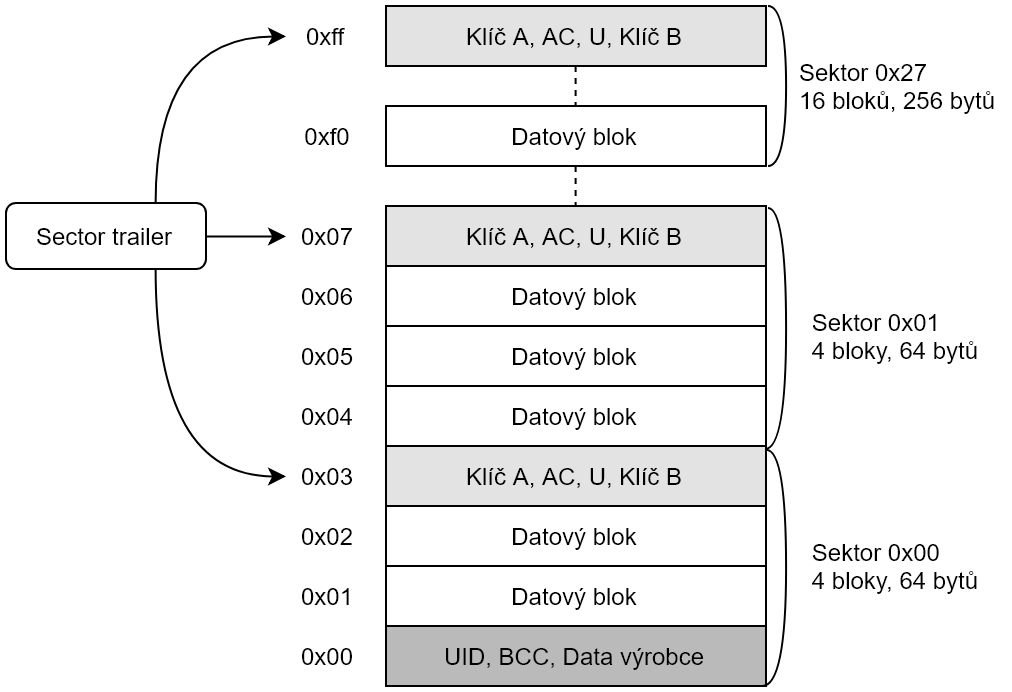
\includegraphics[width=0.6\linewidth,height=180px]{obrazky-figures/MemoryStructure.png}\\[1pt]  
  \caption{Struktura paměti karty Classic\cite{PracticalAttackOnMIFARE}}    
  \label{obrazekStrukturaPametiKarty}
\end{figure*}

\par
Před jakoukoliv operací nad pamětí karty se čtecí zařízení musí nejprve autentizovat proti sektoru se kterým chce pracovat. Každý sektor uzavírá takzvaný sector trailer, speciální datový blok. Obsahuje tajné klíče A a B, které jsou použity při autentizaci. Operace, které je možné nad sektorem provádět, jsou v podmínkách přístupu AC. Poslední částí sector traileru je jeden datový byte U, který nemá definovaný účel. Může však být použit pro uložení dat. Sector trailer má zvláštní  podmínky přístupu. Zatímco klíč A není čitelný nikdy, klíči B se čitelnost nastavit může. V takovém případě se jím nedá autentizovat. Čitelností klíče je myšlen přístup čtecího zařízení k tomuto datovému prostoru s právy pro čtení, karta samotná je může číst bez problémů.
\par
Na datových blocích jsou uložena libovolná data, nebo jsou konfigurovány jako blok s hodnotou (value block). Při použití hodnotového bloku je 4 bytová, podepsaná hodnota uložena dohromady třikrát. Dvakrát normálně a jednou invertovaně, tedy se všemi bity negovanými. Tyto 4 byty mají uložen nejvýznamnější byte vpravo a nejméně významný vlevo ({little-endian}). Na posledních čtyřech bytech je uložena jedno bytová adresa bloku, která může být použita jako ukazatel. Adresa je uložena čtyři krát po sobě, z toho druhý a čtvrtý byte jsou opět negovány\cite{PracticalAttackOnMIFARE}.

\begin{figure*}[ht]\centering
  \centering
  \hspace*{-0.07\linewidth}
  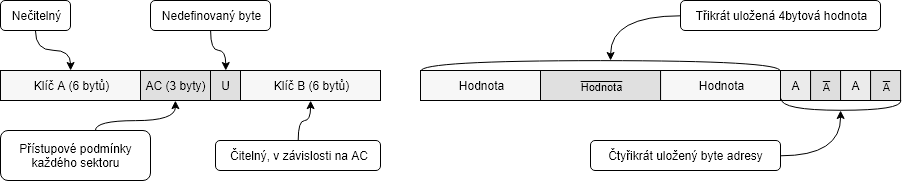
\includegraphics[width=1.1\linewidth,height=1.6in]{obrazky-figures/LogicalStructureBetter.png}\\[1pt]  
  \caption{Struktura paměti sector traileru a bloku s hodnotou\cite{PracticalAttackOnMIFARE}}    
  \label{obrazekStrukturaSpecialnichBloku}
\end{figure*}

Pro manipulace s daty mají karty Classic malou sadu příkazů. Aby mohly být provedeny nad datovým blokem, musí být čtecí zařízení autentizováno pro sektor který tento blok obsahuje. Před každým použitím jakéhokoliv příkazu se kontrolují přístupové podmínky. Ne všechny příkazy mohou být povoleny. Například blok může být nastaven pouze pro čtení, nebo jiný blok s hodnotou může být pouze inkrementován.
\par
Příkazy Read a Write čtou nebo zapisují jeden blok. Ten může být jak datový, tak hodnotový. Příkaz Write může být použit k formátování datového bloku na blok s hodnotou, nebo na zapsání libovolných dat do bloku. Další příkazy jsou povoleny pouze na hodnotových blocích. Jsou to Decrement, Increment, Restore a Transfer. Příkazy Increment a Decrement inkrementují nebo dekrementují hodnotu hodnotového bloku a výsledek vloží do paměťového registru. Příkaz Restore načte do registru hodnotu nezměněnou a příkaz Transfer nahraje hodnotu z registru zpět do stejného, nebo jiného bloku\cite{PracticalAttackOnMIFARE}.
% subsection struktura_paměti (end)

\subsection{CRYPTO1}
Po autentizati je veškerá komunikace mezi čtecím zařízením a kartou šifrována. Pro šifrování se používá proprietární proudová šifra CRYPTO1 navržena přímo firmou NXP\cite{Mifare_Classic_story}. Proudové šifry jsou symetrické šifry kde je důvěrný text neznámé délky (anglicky plaintext) bit po bitu kombinován s proudem pseuhonáhodných šifrovacích bitů (dále jen anglicky keystream). Kombinace se nejčastěji provádí pomocí funkce XOR a jejím výsledkem je zašifrovaný text (cipher text). Šifrovaný text je dešifrován stejnou funkcí a keystreamem. Keystream i důvěrný text musí být stejně dlouhé. Aby bylo možné tohoto dosáhnout s konečnou pamětí, je potřeba keystream generovat. To se děje na základě klíče (anglicky secret key) v generátoru\cite{Stream_ciphers}. Šifra CRYPTO1 jako generátor používá 48 bitový posuvný registr s lineární zpětnou vazbou (dále jen LFSR, z anglického Linear Feedback Shift-register) s generačním polynomem \ref{generatingPolynomial}. Každou periodu hodinového signálu se z dvaceti určitých bitů pomocí filtrační funkce \ref{filterFunction} vypočítá bit keystreamu, a potom se všechny bity registru posunou doleva. Nejlevější bit je zahozen a nový, pravý bit je jako zpětná vazba vypočítán funkcí \ref{feedbackFunction}, kde x je aktuální stav registru. V průběhu inicializace se bere v úvahu také vstupní bit, který je kombinován funkcí XOR s \ref{feedbackFunction}. \cite{Dismantling_Mifare_Classic}.

\begin{multline}
    \label{generatingPolynomial}
    g(x) = x^{48} + x^{43} + x^{39} + x^{38} + x^{36} + x^{34} + x^{33} + x^{31} + x^{29} + x^{24} + \\
     x^{23} + x^{21} + x^{19} + x^{13} + x^{9} + x^{7} + x^{6} + x^{5} + 1  % generating polynomial z dismantling
\end{multline}
\begin{multline}
    \label{feedbackFunction}
    L(x_0, x_1 \dots x_{47}) = x_{0} \oplus x_{5} \oplus x_{9} \oplus x_{10} \oplus x_{12} \oplus x_{14} \oplus x_{15} \oplus x_{17} \oplus x_{19} \oplus x_{24} \oplus \\ 
    x_{25} \oplus x_{27} \oplus x_{29} \oplus x_{35} \oplus x_{39} \oplus x_{41} \oplus x_{42} \oplus x_{43}
\end{multline}
\begin{multline}
    \label{filterFunction}
    f(x_0, x_1 \dots x_{47}) = f_c(f_a(x_{9},x_{11},x_{13},x_{15}),
                               f_b(x_{17},x_{19},x_{21},x_{23}),
                               f_b(x_{25},x_{27},x_{29},x_{31}), \\
                               f_a(x_{33},x_{35},x_{37},x_{39}),
                               f_b(x_{41},x_{43},x_{45},x_{47}))
\end{multline}
\begin{multline}
    \label{filterFunctionC}
    f_c(y_0,y_1,y_2,y_3,y_4) = 
    (y_0 \lor ((y_1 \lor y_4) \land (y_3 \oplus y_4))) \oplus \\
    ((y_0 \oplus(y_1 \land y_3)) \land ((y_2 \oplus y_3) \lor (y_1\land y_4)))
\end{multline}
\begin{equation}
    \label{filterFunctionA}
    f_a(y_0,y_1,y_2,y_3) = 
    ((y_0 \lor y_1) \oplus (y_0 \land y_3)) \oplus (y_2 \land ((y_0 \oplus y_1) \lor y_3))
\end{equation}
\begin{equation}
    \label{filterFunctionB}
    f_b(y_0,y_1,y_2,y_3) = ((y_0 \land y_1) \lor y_2) \oplus ((y_0 \oplus y_1) \land (y_2 \lor y_3))
\end{equation}

\begin{figure*}[ht]\centering
  \centering
  \hspace*{-0.08\linewidth}
  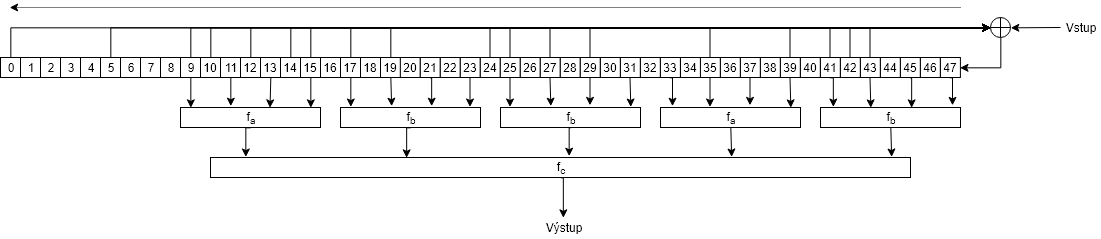
\includegraphics[width=1.1\linewidth,height=120px]{obrazky-figures/StrukturaSifry.png}\\[1pt]  
  \caption{Struktura šifry CRYPTO1\cite{Wirelessly_Pickpocketing}}    
  \label{obrazekStrukturaSifry}
\end{figure*}

\subsection{Komunikační protokol}
\label{komunikacni_protokol}
Komunikace karet MIFARE Classic implementuje standard ISO 14443. Ve čtvrté části se implementace od standardu liší a MIFARE používá svůj vlastní, neveřejný protokol. Po vstupu do blízkosti čtecího zařízení a nabití nastává antikolizní fáze, v níž je karta vybrána. Ta poté posílá své UID \emph{u}. Čtecí zařízení požádá o autentizaci pro specifický sektor a karta mu pošlé výzvu (anglicky challenge) ${n_T}$\footnotemark ve formě takzvané nonce\cite{Wirelessly_Pickpocketing}. Nonce je anglický výraz pro slovo na jedno použití. V kryptografii označuje náhodné číslo použité při komunikaci pouze jednou\cite{Nonce_Based_Encryption}. Od této chvíle je komunikace šifrována, tedy XORována s pseudonáhodným proudem bitů (anglicky keystream). Čtecí zařízení poté odpoví se svou vlastní výzvou ${n_R}$ a odpovědí na výzvu karty ${a_R = suc^{64}(n_T)}$. Autentizace je dokončena odpovědí karty ${a_T = suc^{96}(n_R)}$. Po této odpovědi jsou karta i čtecí zařízení vůči sobě autentizovány\cite{Wirelessly_Pickpocketing}. 
\footnotetext{Notace je zachována stejná jako v \cite{Wirelessly_Pickpocketing}, tedy \emph{T} jako tag, \emph{R} jako reader, \emph{n} jako nonce a \emph{a} jako answer}



\section{Známé zranitelnosti}
Nejjednodušším útokem na chytré karty je takzvaný replay attack. K provedení je nutné z komunikace zachytit UID, které posílá karta, a poté toto stejné UID vysílat. Tento útok lze provést nad systémy, které požadují pouze odeslané UID. Karty MIFARE Classic jsou složitější. Útoky na ně se zaměřují na chyby, nebo zranitelné místa v jejich návrhu\cite{Mifare_Classic_story}.
\par
%Krátké šifrovací klíče
Pro šifrování karet se používají 48 bitové klíče. Tato délka klíčů je ale příliš malá na to, aby zabránila úspěšnému brute force útoku v dosažitelném čase. Proto bylo zavedeno zpoždění v komunikaci a v autentizaci. Každý pokus by trval 6 milisekund. Díky této kompenzaci by online brute force útok na jeden sektor, prohledávajíci všech $2^{48}$ možných klíčů, trval více než 44 tisíc let. Odhalení algoritmu šifry CRYPTO1 umožnilo provést offline brute force útok. V takovém případě útočník nemusí komunikovat se zařízením pod útokem. Stačí mu pouze záznam komunikace, tím se eliminuje zavedené spoždění. V prosinci 2007 Nohl a Plötz uvedli, že zařízení za 100\$ dokáže najít klíč přibližně za týden. Tato doba lze dál zkrátit přidáním paměti\cite{Cryptanalisis}.
\par
%předvídatelné nonce
Aby mohly kryptografické protokoly poskytovat správné zabezpečení, je pro ně zásadní dostatečný generátor pseudonáhodných čísel. Čísla pro MIFARE Classic generuje 16 bitový LFSR. Výzvy $n_T$(nonce, viz. \ref{komunikacni_protokol}) použité při autentizaci jsou ale 32 bitové. To znamená, že první polovina $n_T$ určuje její zbytek. Sekvence všech výzev se opakuje každých $2^{16} - 1$ cyklů\cite{Cryptanalisis}. Cyklus generátoru karty je rozdílný od čtecího zařízení. Zatímco karta mění stav každou periodu hodinového signálu, čtecí zařízení aktualizuje stav jen při volání generátoru\cite{Dismantling_Mifare_Classic}. Generátor v kartě se resetuje do původního stavu při každém nastartování karty. Výzva poslaná kartou je tedy podmíněna pouze časem mezi zapnutím elektromagnetického pole k nabití karty a momentem odeslání žádosti o autentizaci. Autentizace je tedy zbavena jakékoliv náhodnosti. \parÚtočník s fyzickým přístupem ke kartě ji může "přinutit" k odeslání vždy stejné výzvy. K tomu je potřeba po každém pokusu vypnout elektromagnetické pole (zhruba na 30$\mu$s), aby se vybily všechny kondenzátory, znovu zapnout pole, počkat konstantní čas před odesláním požadavku o autentizaci. Druhý způsob spočívá v čekání mezi znovuodesláním požadavku přesně stanovený čas \emph{t}. Stav generátoru pseudonáhodných čísel se mění každých 9,44$\mu$s. Na vystřídání všech stavů tak stačí pouze $(2^{16} - 1) * 9,44\mu$s $= 618,650ms$. Velikost výzvy je dvojnásobná oproti LFSR, výsledný čas \emph{t} je tedy poloviční $t = 618ms/2 = 309ms$ \cite{Wirelessly_Pickpocketing}. V novější verzi karet Classic EV1 je tento nedostatek odstraněn nahrazením generátoru pseudonáhodných čísel generátorem náhodných čísel\cite{MIFARE_Classic_Official_about}.
%\subsection{Získání stavu posuvného registru}

%\subsection{Navrácení stavu posuvného registru}

%\subsection{Vstup filtrační funkce}

%\subsection{Paritní bity}
%Smart Card Security \cite{Smart_Cards_Tokens_Security}{ - str. 224-254}


%                               NADPIS                      
\chapter{Zařízení Chameleon Mini}
\label{zarizeni_chameleon_mini}







\chapter{Závěr}
\label{zaver}


%===============================================================================
